% CENTRAL OBSERVABILITY DESIGN VISUALS
% One shared SQL Server store, two ingestion paths — generated for deep
% technical review. Same visual language as METADATA_DESIGN_VISUALS.tex /
% STS2_DESIGN_VISUALS_V2.tex.
% Compile: pdflatex CENTRAL_OBSERVABILITY_VISUALS.tex (twice)
% NOTE: authored without local TeX tooling — pages scale via \adjustbox;
% any compile complaint should be a one-line fix, not structural.
\documentclass[10pt]{article}
\usepackage[a4paper,landscape,margin=10mm]{geometry}
\usepackage[T1]{fontenc}
\usepackage[sc]{mathpazo}
\usepackage{microtype}
\usepackage{tikz}
\usetikzlibrary{arrows.meta,positioning,fit,calc,backgrounds,shapes.geometric,shapes.multipart,decorations.pathreplacing,matrix}
\usepackage{xcolor}
\usepackage{adjustbox}
\usepackage{hyperref}
\hypersetup{hidelinks}
\pagestyle{empty}
\setlength{\parindent}{0pt}

\definecolor{runtime}{HTML}{EAF0FF}   % central store
\definecolor{core}{HTML}{EAF8EC}      % producers / ground truth
\definecolor{journal}{HTML}{FFF0EE}   % writers / transport
\definecolor{observer}{HTML}{F6EDFA}  % readers / analysis
\definecolor{edge}{HTML}{FFF5E6}      % CI / automation
\definecolor{external}{HTML}{F4F4F4}  % external / optional
\definecolor{risk}{HTML}{FFE3E3}
\definecolor{good}{HTML}{E2F5E7}
\definecolor{policy}{HTML}{E8F7F5}    % privacy / policy gates
\definecolor{ink}{HTML}{263238}
\definecolor{muted}{HTML}{607D8B}
\definecolor{blue}{HTML}{3F6FB5}
\definecolor{red}{HTML}{B54A4A}
\definecolor{purple}{HTML}{7A4E9B}
\definecolor{orange}{HTML}{B56A24}
\definecolor{green}{HTML}{39784A}

\tikzset{
  >=Latex,
  every node/.style={font=\small,text=ink},
  box/.style={draw=ink!65,rounded corners=2.5pt,fill=runtime,minimum height=11mm,minimum width=35mm,align=center,inner sep=4pt},
  prodbox/.style={box,fill=core},
  writebox/.style={box,fill=journal,draw=red!75},
  readbox/.style={box,fill=observer,draw=purple!70},
  cibox/.style={box,fill=edge,draw=orange!75},
  extbox/.style={box,fill=external,dashed},
  policybox/.style={box,fill=policy,draw=green!70},
  riskbox/.style={box,fill=risk,draw=red!80},
  goodbox/.style={box,fill=good,draw=green!75},
  tinybox/.style={draw=ink!60,rounded corners=2pt,fill=white,align=center,inner sep=3pt,font=\footnotesize},
  state/.style={draw=ink!65,rounded corners=6pt,fill=runtime,minimum width=29mm,minimum height=10mm,align=center},
  term/.style={state,fill=good},
  badstate/.style={state,fill=risk,draw=red!80},
  arrow/.style={->,very thick,draw=ink!75},
  async/.style={->,thick,dashed,draw=purple},
  write/.style={->,very thick,draw=red},
  effect/.style={->,very thick,draw=orange},
  policyarr/.style={->,very thick,draw=green},
  fail/.style={->,very thick,dashed,draw=red},
  note/.style={draw=ink!30,rounded corners=2pt,fill=white,align=left,inner sep=5pt,font=\footnotesize,text width=70mm},
  pill/.style={draw=ink!45,rounded corners=7pt,fill=white,inner xsep=6pt,inner ysep=2pt,font=\footnotesize\bfseries},
  label/.style={font=\footnotesize,align=center,fill=white,inner sep=1.5pt},
}
\newcommand{\code}[1]{\texttt{#1}}
\newcommand{\pagehead}[2]{%
  \begin{minipage}[t]{0.73\linewidth}
    {\Large\bfseries #1}\\[-1mm]
    {\small\color{muted}#2}
  \end{minipage}\hfill
  \begin{minipage}[t]{0.25\linewidth}\raggedleft
    {\footnotesize Central observability --- proposed design}\\
    {\scriptsize vscode-mssql 091b6712b $\cdot$ perftest a01dc2c}
  \end{minipage}
  \vspace{3mm}\hrule\vspace{4mm}
}
\newcommand{\legend}{%
\tikz[baseline=-0.7ex]\node[prodbox,minimum width=7mm,minimum height=4mm,inner sep=1pt]{}; producers/ground truth\quad
\tikz[baseline=-0.7ex]\node[writebox,minimum width=7mm,minimum height=4mm,inner sep=1pt]{}; writers/transport\quad
\tikz[baseline=-0.7ex]\node[box,minimum width=7mm,minimum height=4mm,inner sep=1pt]{}; central store\quad
\tikz[baseline=-0.7ex]\node[readbox,minimum width=7mm,minimum height=4mm,inner sep=1pt]{}; readers\quad
\tikz[baseline=-0.7ex]\node[cibox,minimum width=7mm,minimum height=4mm,inner sep=1pt]{}; CI\quad
\tikz[baseline=-0.7ex]\node[policybox,minimum width=7mm,minimum height=4mm,inner sep=1pt]{}; policy gate
}

\begin{document}

% =====================================================================
% PAGE 1 — SYSTEM LANDSCAPE
% =====================================================================
\pagehead{P1. One store, two ingestion paths}
{Ad-hoc team uploads (Debug Console, product data plane) and official CI/CD results (perftest push) write ONE schema through ONE vendored contract.}
\legend\par\vspace{4mm}

\begin{adjustbox}{max width=\linewidth,max height=0.82\textheight,center}
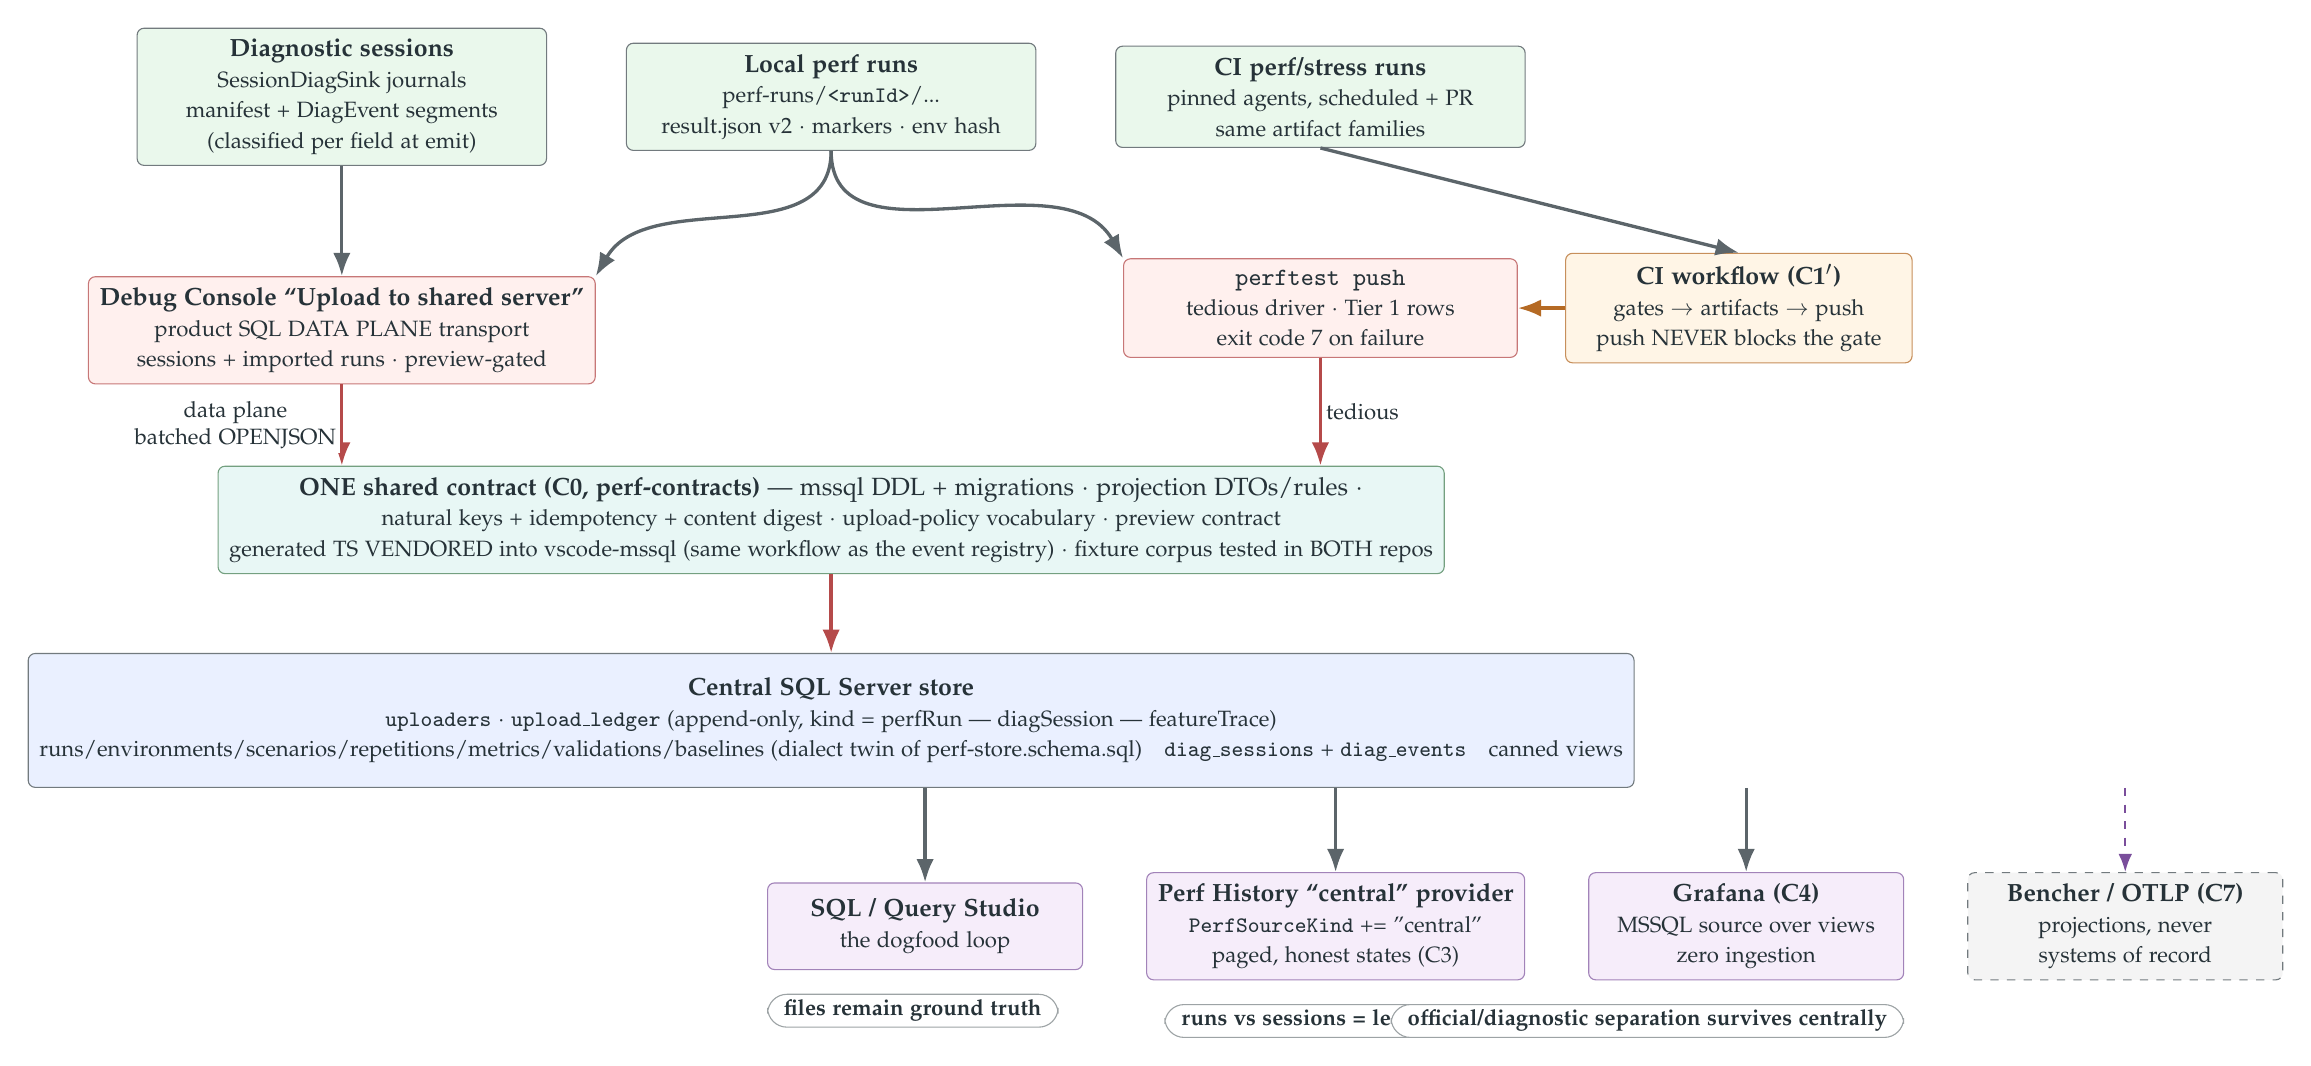
\begin{tikzpicture}[node distance=7mm and 10mm]

% producers row
\node[prodbox,minimum width=52mm] (sessions)
{\textbf{Diagnostic sessions}\\\footnotesize SessionDiagSink journals\\\footnotesize manifest + DiagEvent segments\\\footnotesize (classified per field at emit)};
\node[prodbox,minimum width=52mm,right=of sessions] (localruns)
{\textbf{Local perf runs}\\\footnotesize perf-runs/\code{<runId>}/...\\\footnotesize result.json v2 $\cdot$ markers $\cdot$ env hash};
\node[prodbox,minimum width=52mm,right=of localruns] (ciruns)
{\textbf{CI perf/stress runs}\\\footnotesize pinned agents, scheduled + PR\\\footnotesize same artifact families};

% writers
\node[writebox,minimum width=58mm,below=14mm of sessions]
(dcupload)
{\textbf{Debug Console ``Upload to shared server''}\\\footnotesize product SQL DATA PLANE transport\\\footnotesize sessions + imported runs $\cdot$ preview-gated};
\node[writebox,minimum width=50mm,below=14mm of ciruns] (push)
{\textbf{\code{perftest push}}\\\footnotesize tedious driver $\cdot$ Tier 1 rows\\\footnotesize exit code 7 on failure};
\node[cibox,minimum width=44mm,right=6mm of push] (workflow)
{\textbf{CI workflow (C1$'$)}\\\footnotesize gates $\to$ artifacts $\to$ push\\\footnotesize push NEVER blocks the gate};

% contract
\node[policybox,minimum width=104mm,below=12mm of $(dcupload.south)!0.5!(push.south)$] (contract)
{\textbf{ONE shared contract (C0, perf-contracts)} — mssql DDL + migrations $\cdot$ projection DTOs/rules $\cdot$\\\footnotesize
natural keys + idempotency + content digest $\cdot$ upload-policy vocabulary $\cdot$ preview contract\\\footnotesize
generated TS VENDORED into vscode-mssql (same workflow as the event registry) $\cdot$ fixture corpus tested in BOTH repos};

% store
\node[box,minimum width=150mm,minimum height=17mm,below=10mm of contract] (store)
{\textbf{Central SQL Server store}\\\footnotesize
\code{uploaders} $\cdot$ \code{upload\_ledger} (append-only, kind = perfRun | diagSession | featureTrace)\\\footnotesize
runs/environments/scenarios/repetitions/metrics/validations/baselines (dialect twin of perf-store.schema.sql)\quad
\code{diag\_sessions} + \code{diag\_events}\quad canned views};

% readers
\node[readbox,minimum width=40mm,below left=12mm and -32mm of store.south] (sqlread)
{\textbf{SQL / Query Studio}\\\footnotesize the dogfood loop};
\node[readbox,minimum width=48mm,right=8mm of sqlread] (provider)
{\textbf{Perf History ``central'' provider}\\\footnotesize \code{PerfSourceKind} += "central"\\\footnotesize paged, honest states (C3)};
\node[readbox,minimum width=40mm,right=8mm of provider] (grafana)
{\textbf{Grafana (C4)}\\\footnotesize MSSQL source over views\\\footnotesize zero ingestion};
\node[extbox,minimum width=40mm,right=8mm of grafana] (proj)
{\textbf{Bencher / OTLP (C7)}\\\footnotesize projections, never\\\footnotesize systems of record};

% arrows
\draw[arrow] (sessions.south) -- (dcupload.north);
\draw[arrow] (localruns.south) to[out=-90,in=60] (dcupload.north east);
\draw[arrow] (localruns.south) to[out=-90,in=120] (push.north west);
\draw[arrow] (ciruns.south) -- (workflow.north);
\draw[effect] (workflow.west) -- (push.east);
\draw[write] (dcupload.south) -- node[label,left]{data plane\\\footnotesize batched OPENJSON} (contract.north -| dcupload.south);
\draw[write] (push.south) -- node[label,right]{tedious} (contract.north -| push.south);
\draw[write] (contract.south) -- (store.north);
\draw[arrow] (store.south -| sqlread.north) -- (sqlread.north);
\draw[arrow] (store.south -| provider.north) -- (provider.north);
\draw[arrow] (store.south -| grafana.north) -- (grafana.north);
\draw[async] (store.south -| proj.north) -- (proj.north);

% pills
\node[pill,below=3mm of sqlread.south west,anchor=north west] {files remain ground truth};
\node[pill,below=3mm of provider.south,anchor=north] {runs vs sessions = ledger \code{kind}};
\node[pill,below=3mm of grafana.south east,anchor=north east] {official/diagnostic separation survives centrally};

\end{tikzpicture}
\end{adjustbox}

\newpage
% =====================================================================
% PAGE 2 — DATA MODEL: THE INGEST SPINE
% =====================================================================
\pagehead{P2. The ingest spine: ledger, kinds, shared dimensions}
{``Runs vs.\ sessions'' is a first-class kind over shared dimensions — aggregation is a GROUP BY, not a federation project.}
\legend\par\vspace{4mm}

\begin{adjustbox}{max width=\linewidth,max height=0.82\textheight,center}
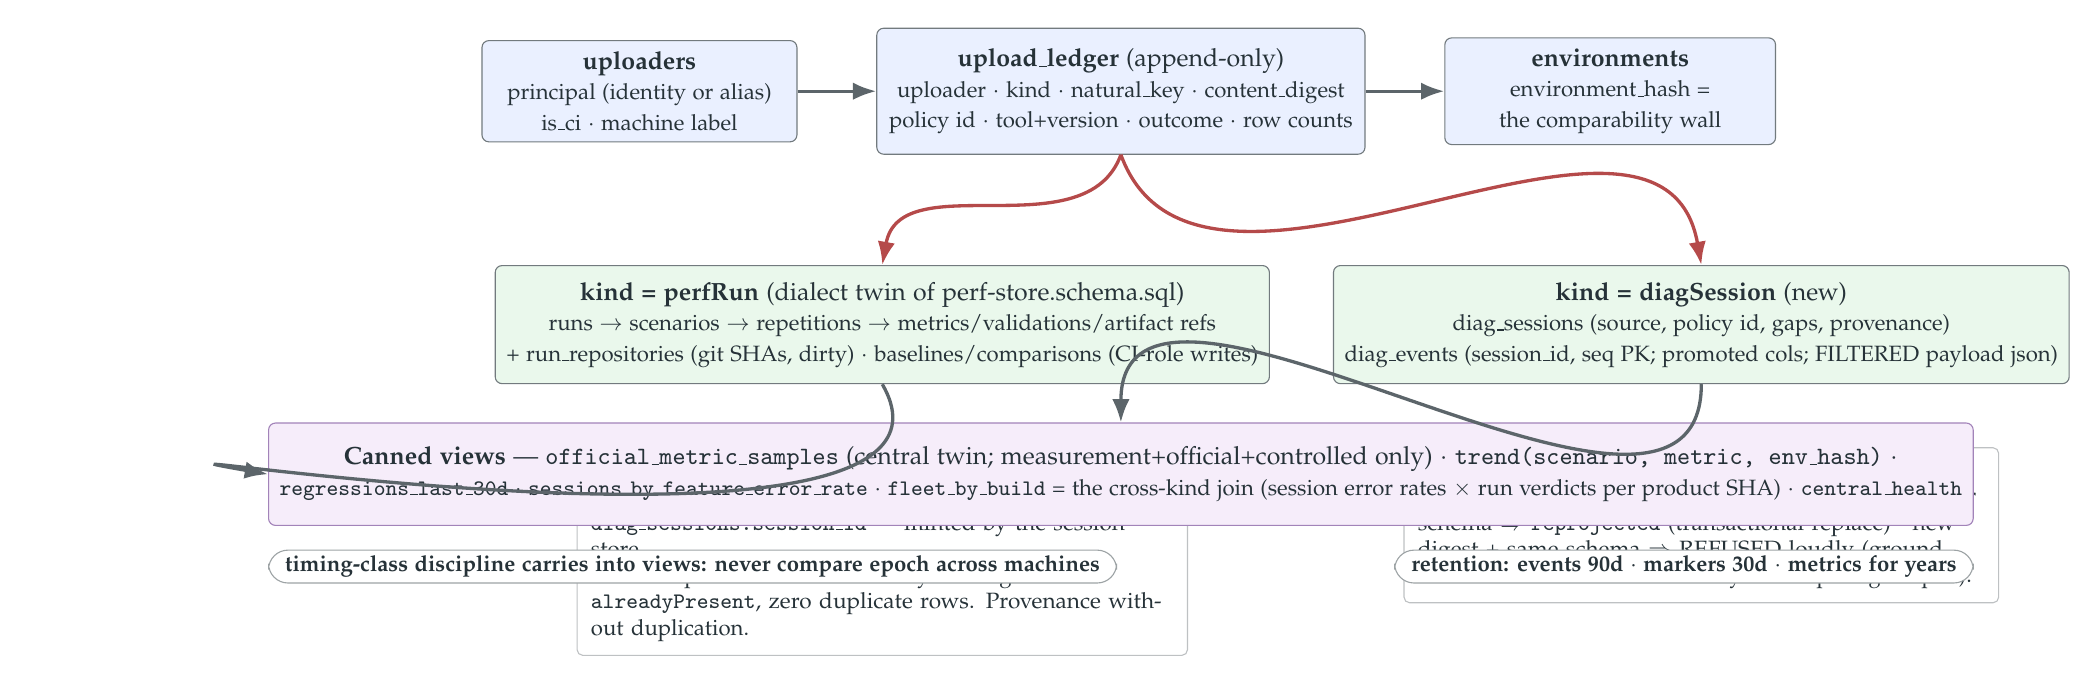
\begin{tikzpicture}[node distance=7mm and 9mm]

\node[box,minimum width=62mm,minimum height=16mm] (ledger)
{\textbf{upload\_ledger} (append-only)\\\footnotesize uploader $\cdot$ kind $\cdot$ natural\_key $\cdot$ content\_digest\\\footnotesize policy id $\cdot$ tool+version $\cdot$ outcome $\cdot$ row counts};
\node[box,minimum width=40mm,left=10mm of ledger] (uploaders)
{\textbf{uploaders}\\\footnotesize principal (identity or alias)\\\footnotesize is\_ci $\cdot$ machine label};
\node[box,minimum width=42mm,right=10mm of ledger] (envs)
{\textbf{environments}\\\footnotesize environment\_hash =\\\footnotesize the comparability wall};

\draw[arrow] (uploaders) -- (ledger);
\draw[arrow] (ledger) -- (envs);

% run kind
\node[prodbox,minimum width=74mm,minimum height=15mm,below left=14mm and -50mm of ledger]
(runkind)
{\textbf{kind = perfRun} (dialect twin of perf-store.schema.sql)\\\footnotesize runs $\to$ scenarios $\to$ repetitions $\to$ metrics/validations/artifact refs\\\footnotesize + run\_repositories (git SHAs, dirty) $\cdot$ baselines/comparisons (CI-role writes)};
% session kind
\node[prodbox,minimum width=72mm,minimum height=15mm,right=8mm of runkind]
(sesskind)
{\textbf{kind = diagSession} (new)\\\footnotesize diag\_sessions (source, policy id, gaps, provenance)\\\footnotesize diag\_events (session\_id, seq PK; promoted cols; FILTERED payload json)};

\draw[write] (ledger.south) to[out=-110,in=80] (runkind.north);
\draw[write] (ledger.south) to[out=-70,in=100] (sesskind.north);

% keys note
\node[note,below=8mm of runkind,text width=74mm]
{\textbf{Natural keys (global UNIQUE, not per uploader):}\\
\code{runs.run\_id} — timestamp+hash, minted by the harness\\
\code{diag\_sessions.session\_id} — minted by the session store\\
Second uploader of the same key $\Rightarrow$ ledger \code{alreadyPresent}, zero duplicate rows. Provenance without duplication.};

\node[note,below=8mm of sesskind,text width=72mm]
{\textbf{content\_digest decides re-push semantics:}\\
same digest $\Rightarrow$ no-op $\cdot$ new digest + NEWER projector schema $\Rightarrow$ \code{reprojected} (transactional replace) $\cdot$ new digest + same schema $\Rightarrow$ REFUSED loudly (ground truth never mutates under a key — tampering-shaped).};

% views
\node[readbox,minimum width=150mm,minimum height=13mm,below=34mm of ledger]
(views)
{\textbf{Canned views} — \code{official\_metric\_samples} (central twin; measurement+official+controlled only) $\cdot$ \code{trend(scenario, metric, env\_hash)} $\cdot$\\\footnotesize \code{regressions\_last\_30d} $\cdot$ \code{sessions\_by\_feature\_error\_rate} $\cdot$ \textbf{\code{fleet\_by\_build}} = the cross-kind join (session error rates $\times$ run verdicts per product SHA) $\cdot$ \code{central\_health}};
\draw[arrow] (runkind.south) to[out=-60,in=170] (views.west);
\draw[arrow] (sesskind.south) to[out=-90,in=90] (views.north);

\node[pill,below=3mm of views.south west,anchor=north west] {timing-class discipline carries into views: never compare epoch across machines};
\node[pill,below=3mm of views.south east,anchor=north east] {retention: events 90d $\cdot$ markers 30d $\cdot$ metrics for years};

\end{tikzpicture}
\end{adjustbox}

\newpage
% =====================================================================
% PAGE 3 — IDEMPOTENT UPLOAD PROTOCOL + POLICY GATE
% =====================================================================
\pagehead{P3. Upload protocol: policy gate, then idempotent landing}
{The preview IS the projection (dry-run). Every outcome is a ledger row; nothing lands without classification filtering.}
\legend\par\vspace{4mm}

\begin{adjustbox}{max width=\linewidth,max height=0.82\textheight,center}
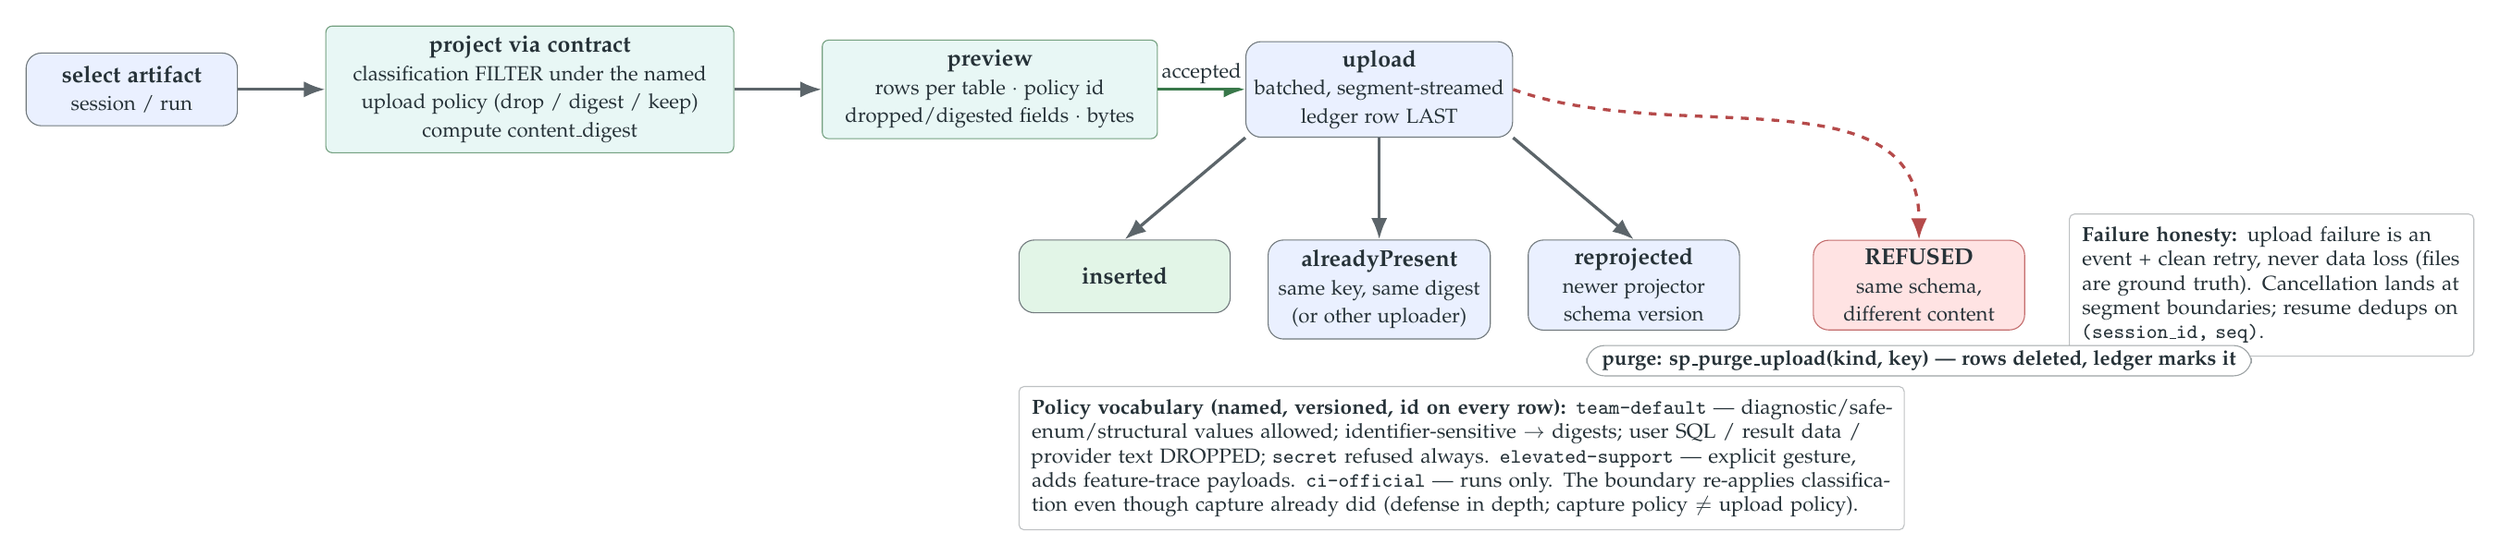
\begin{tikzpicture}[node distance=8mm and 12mm]

\node[state] (start) {\textbf{select artifact}\\\footnotesize session / run};
\node[policybox,minimum width=56mm,right=of start] (project)
{\textbf{project via contract}\\\footnotesize classification FILTER under the named\\\footnotesize upload policy (drop / digest / keep)\\\footnotesize compute content\_digest};
\node[policybox,minimum width=46mm,right=of project] (preview)
{\textbf{preview}\\\footnotesize rows per table $\cdot$ policy id\\\footnotesize dropped/digested fields $\cdot$ bytes};
\node[state,right=of preview] (send) {\textbf{upload}\\\footnotesize batched, segment-streamed\\\footnotesize ledger row LAST};

\draw[arrow] (start) -- (project);
\draw[arrow] (project) -- (preview);
\draw[policyarr] (preview) -- node[label,above]{accepted} (send);

% outcomes
\node[term,below left=14mm and 2mm of send] (inserted) {\textbf{inserted}};
\node[goodbox,state,below=14mm of send] (already) {\textbf{alreadyPresent}\\\footnotesize same key, same digest\\\footnotesize (or other uploader)};
\node[state,below right=14mm and 2mm of send] (reproj) {\textbf{reprojected}\\\footnotesize newer projector\\\footnotesize schema version};
\node[badstate,right=10mm of reproj] (refused) {\textbf{REFUSED}\\\footnotesize same schema,\\\footnotesize different content};

\draw[arrow] (send.south west) -- (inserted.north);
\draw[arrow] (send.south) -- (already.north);
\draw[arrow] (send.south east) -- (reproj.north);
\draw[fail] (send.east) to[out=-20,in=90] (refused.north);

\node[note,below=10mm of inserted.south west,anchor=north west,text width=118mm]
{\textbf{Policy vocabulary (named, versioned, id on every row):} \code{team-default} — diagnostic/safe-enum/structural values allowed; identifier-sensitive $\to$ digests; user SQL / result data / provider text DROPPED; \code{secret} refused always. \code{elevated-support} — explicit gesture, adds feature-trace payloads. \code{ci-official} — runs only. The boundary re-applies classification even though capture already did (defense in depth; capture policy $\neq$ upload policy).};

\node[note,right=6mm of refused.east,anchor=west,text width=52mm]
{\textbf{Failure honesty:} upload failure is an event + clean retry, never data loss (files are ground truth). Cancellation lands at segment boundaries; resume dedups on \code{(session\_id, seq)}.};

\node[pill,below=2mm of refused.south,anchor=north] {purge: sp\_purge\_upload(kind, key) — rows deleted, ledger marks it};

\end{tikzpicture}
\end{adjustbox}

\newpage
% =====================================================================
% PAGE 4 — THE TWO WRITER LANES
% =====================================================================
\pagehead{P4. Writer lanes: product data plane vs CLI, one contract between them}
{Same projection code path shape on both sides; the fixture corpus pins byte-equal rows so the writers cannot drift.}
\legend\par\vspace{4mm}

\begin{adjustbox}{max width=\linewidth,max height=0.82\textheight,center}
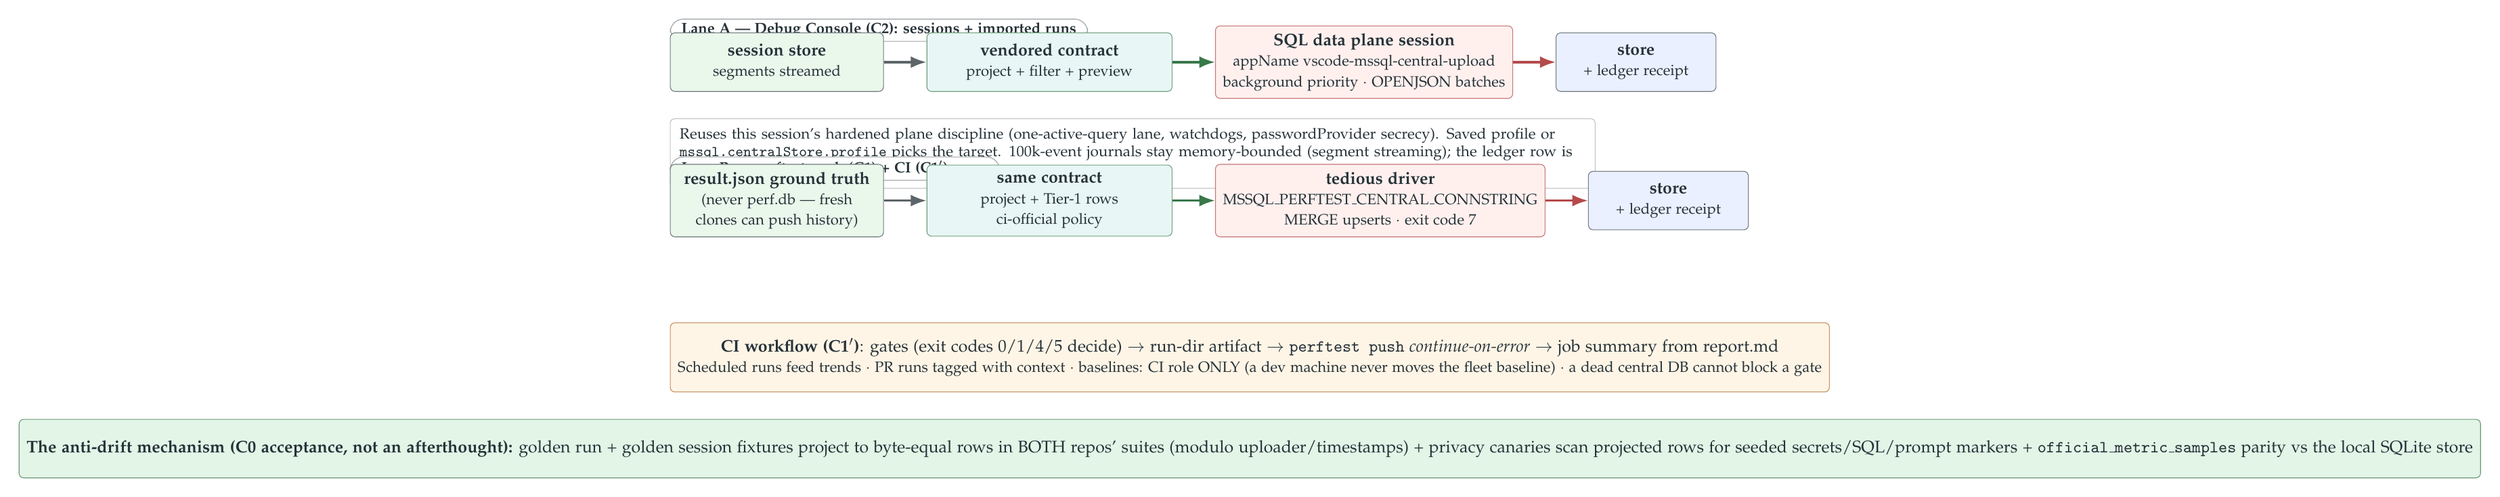
\begin{tikzpicture}[node distance=6mm and 10mm]

% Lane A: Debug Console
\node[pill] (lanea) {Lane A — Debug Console (C2): sessions + imported runs};
\node[prodbox,minimum width=40mm,below=6mm of lanea.west,anchor=west] (a1)
{\textbf{session store}\\\footnotesize segments streamed};
\node[policybox,minimum width=46mm,right=8mm of a1] (a2)
{\textbf{vendored contract}\\\footnotesize project + filter + preview};
\node[writebox,minimum width=48mm,right=8mm of a2] (a3)
{\textbf{SQL data plane session}\\\footnotesize appName vscode-mssql-central-upload\\\footnotesize background priority $\cdot$ OPENJSON batches};
\node[box,minimum width=30mm,right=8mm of a3] (a4) {\textbf{store}\\\footnotesize + ledger receipt};
\draw[arrow] (a1) -- (a2);
\draw[policyarr] (a2) -- (a3);
\draw[write] (a3) -- (a4);

\node[note,below=5mm of a1.south west,anchor=north west,text width=170mm]
{Reuses this session's hardened plane discipline (one-active-query lane, watchdogs, passwordProvider secrecy). Saved profile or \code{mssql.centralStore.profile} picks the target. 100k-event journals stay memory-bounded (segment streaming); the ledger row is written LAST — the upload's ``manifest-last''.};

% Lane B: CLI/CI
\node[pill,below=26mm of lanea.west,anchor=west] (laneb) {Lane B — perftest push (C1) + CI (C1$'$): runs};
\node[prodbox,minimum width=40mm,below=6mm of laneb.west,anchor=west] (b1)
{\textbf{result.json ground truth}\\\footnotesize (never perf.db — fresh\\\footnotesize clones can push history)};
\node[policybox,minimum width=46mm,right=8mm of b1] (b2)
{\textbf{same contract}\\\footnotesize project + Tier-1 rows\\\footnotesize ci-official policy};
\node[writebox,minimum width=48mm,right=8mm of b2] (b3)
{\textbf{tedious driver}\\\footnotesize MSSQL\_PERFTEST\_CENTRAL\_CONNSTRING\\\footnotesize MERGE upserts $\cdot$ exit code 7};
\node[box,minimum width=30mm,right=8mm of b3] (b4) {\textbf{store}\\\footnotesize + ledger receipt};
\draw[arrow] (b1) -- (b2);
\draw[policyarr] (b2) -- (b3);
\draw[write] (b3) -- (b4);

\node[cibox,minimum width=170mm,minimum height=13mm,below=16mm of b1.south west,anchor=north west]
(ci)
{\textbf{CI workflow (C1$'$)}: gates (exit codes 0/1/4/5 decide) $\to$ run-dir artifact $\to$ \code{perftest push} \emph{continue-on-error} $\to$ job summary from report.md\\\footnotesize
Scheduled runs feed trends $\cdot$ PR runs tagged with context $\cdot$ baselines: CI role ONLY (a dev machine never moves the fleet baseline) $\cdot$ a dead central DB cannot block a gate};

\node[goodbox,minimum width=170mm,minimum height=11mm,below=5mm of ci]
(fixtures)
{\textbf{The anti-drift mechanism (C0 acceptance, not an afterthought):} golden run + golden session fixtures project to byte-equal rows in BOTH repos' suites (modulo uploader/timestamps) + privacy canaries scan projected rows for seeded secrets/SQL/prompt markers + \code{official\_metric\_samples} parity vs the local SQLite store};

\end{tikzpicture}
\end{adjustbox}

\newpage
% =====================================================================
% PAGE 5 — BUILD PLAN + DECISIONS
% =====================================================================
\pagehead{P5. Build plan (C0--C7) and the decisions this review must settle}
{C0$\to$C1$\to$C1$'$ run independently of product work; C2 is the first product-side batch; everything downstream needs data first.}
\legend\par\vspace{4mm}

\begin{adjustbox}{max width=\linewidth,max height=0.82\textheight,center}
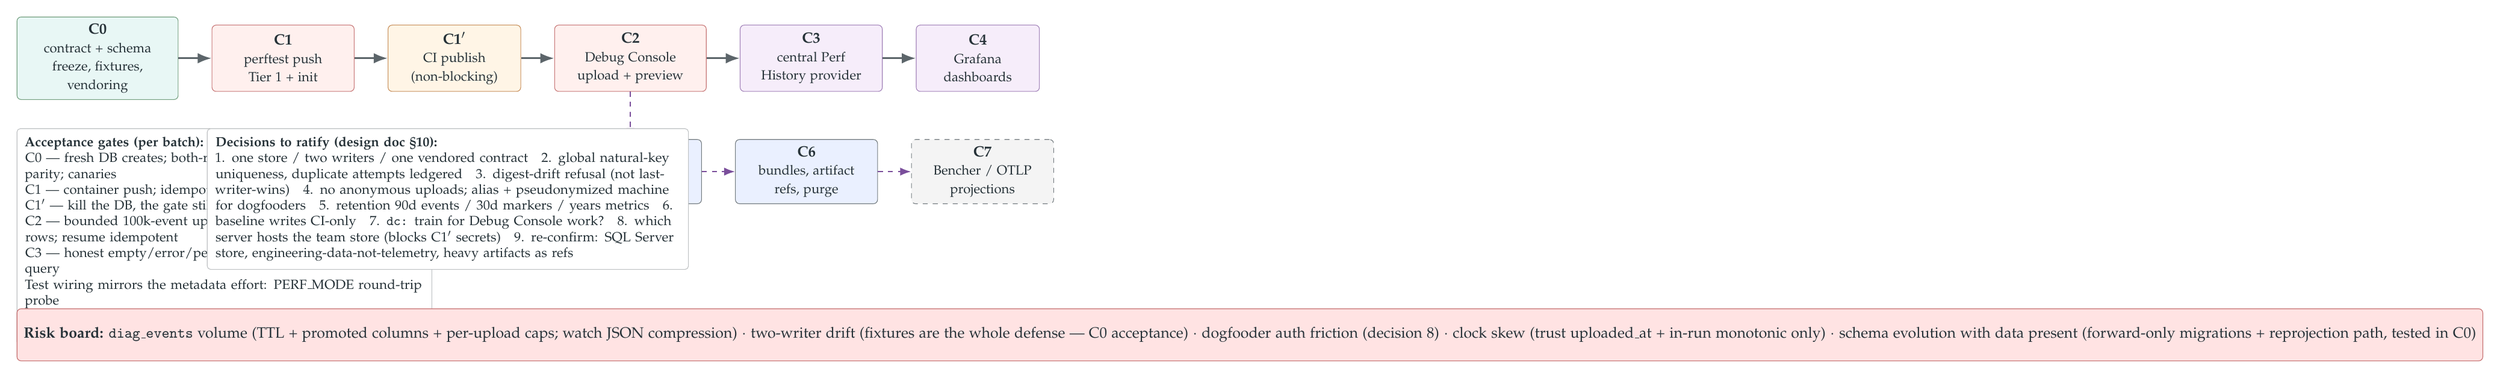
\begin{tikzpicture}[node distance=5mm and 7mm]

\node[policybox,minimum width=34mm,minimum height=14mm] (c0) {\textbf{C0}\\\footnotesize contract + schema\\\footnotesize freeze, fixtures,\\\footnotesize vendoring};
\node[writebox,minimum width=30mm,minimum height=14mm,right=of c0] (c1) {\textbf{C1}\\\footnotesize perftest push\\\footnotesize Tier 1 + init};
\node[cibox,minimum width=28mm,minimum height=14mm,right=of c1] (c1p) {\textbf{C1$'$}\\\footnotesize CI publish\\\footnotesize (non-blocking)};
\node[writebox,minimum width=32mm,minimum height=14mm,right=of c1p] (c2) {\textbf{C2}\\\footnotesize Debug Console\\\footnotesize upload + preview};
\node[readbox,minimum width=30mm,minimum height=14mm,right=of c2] (c3) {\textbf{C3}\\\footnotesize central Perf\\\footnotesize History provider};
\node[readbox,minimum width=26mm,minimum height=14mm,right=of c3] (c4) {\textbf{C4}\\\footnotesize Grafana\\\footnotesize dashboards};

\node[box,minimum width=30mm,minimum height=12mm,below=10mm of c2] (c5) {\textbf{C5}\\\footnotesize markers + SQL\\\footnotesize activity, TTL jobs};
\node[box,minimum width=30mm,minimum height=12mm,right=of c5] (c6) {\textbf{C6}\\\footnotesize bundles, artifact\\\footnotesize refs, purge};
\node[extbox,minimum width=30mm,minimum height=12mm,right=of c6] (c7) {\textbf{C7}\\\footnotesize Bencher / OTLP\\\footnotesize projections};

\draw[arrow] (c0) -- (c1);
\draw[arrow] (c1) -- (c1p);
\draw[arrow] (c1p) -- (c2);
\draw[arrow] (c2) -- (c3);
\draw[arrow] (c3) -- (c4);
\draw[async] (c2.south) to[out=-90,in=90] (c5.north);
\draw[async] (c5) -- (c6);
\draw[async] (c6) -- (c7);

\node[note,below=6mm of c0.south west,anchor=north west,text width=84mm]
{\textbf{Acceptance gates (per batch):}\\
C0 — fresh DB creates; both-repo fixture parity; official-view parity; canaries\\
C1 — container push; idempotent re-push; digest-drift refusal\\
C1$'$ — kill the DB, the gate still gates\\
C2 — bounded 100k-event upload; preview counts == landed rows; resume idempotent\\
C3 — honest empty/error/permission states; trend parity vs CLI query\\
Test wiring mirrors the metadata effort: PERF\_MODE round-trip probe\\
(\code{mssql.perf.centralUploadRoundTrip}) + a perftest scenario over it.};

\node[note,right=6mm of c0.south east,anchor=north west,yshift=-6mm,text width=98mm]
{\textbf{Decisions to ratify (design doc §10):}\\
1. one store / two writers / one vendored contract\quad
2. global natural-key uniqueness, duplicate attempts ledgered\quad
3. digest-drift refusal (not last-writer-wins)\quad
4. no anonymous uploads; alias + pseudonymized machine for dogfooders\quad
5. retention 90d events / 30d markers / years metrics\quad
6. baseline writes CI-only\quad
7. \code{dc:} train for Debug Console work?\quad
8. which server hosts the team store (blocks C1$'$ secrets)\quad
9. re-confirm: SQL Server store, engineering-data-not-telemetry, heavy artifacts as refs};

\node[riskbox,minimum width=178mm,minimum height=11mm,below=44mm of c0.south west,anchor=north west]
(risks)
{\textbf{Risk board:} \code{diag\_events} volume (TTL + promoted columns + per-upload caps; watch JSON compression) $\cdot$ two-writer drift (fixtures are the whole defense — C0 acceptance) $\cdot$ dogfooder auth friction (decision 8) $\cdot$ clock skew (trust uploaded\_at + in-run monotonic only) $\cdot$ schema evolution with data present (forward-only migrations + reprojection path, tested in C0)};

\end{tikzpicture}
\end{adjustbox}

\end{document}
